\documentclass{standalone}
\usepackage{tikz}
\usetikzlibrary{patterns, positioning}

\begin{document}
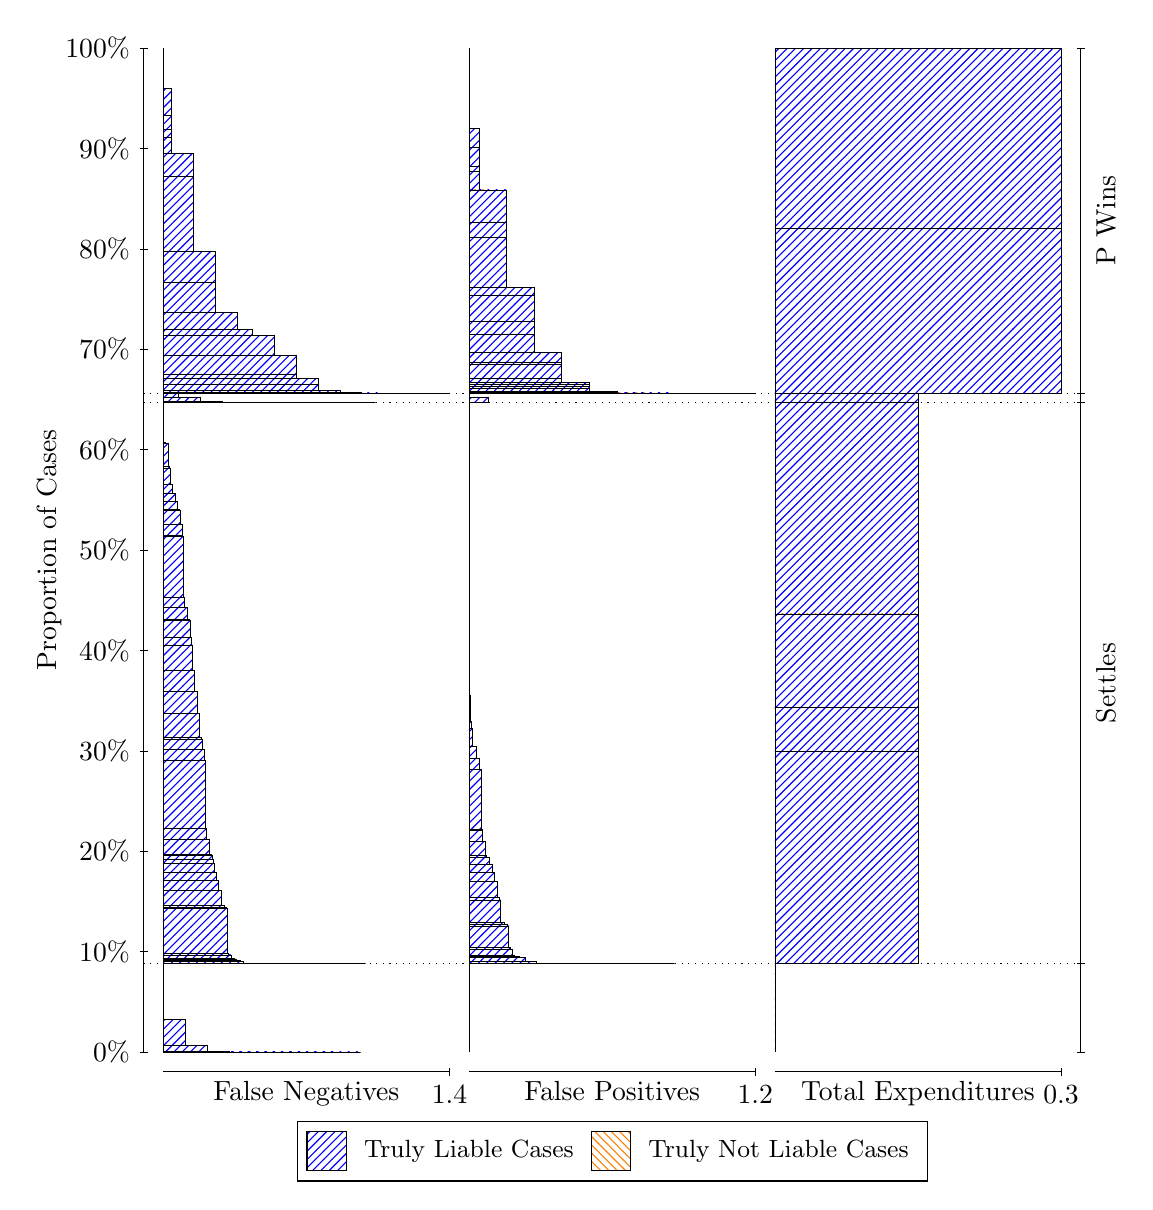
\begin{tikzpicture}
\draw[black, very thin] (1.5,1.75) -- (1.5,14.5);
\node[rotate=90, anchor=center] at (0.3, 8.125) {Proportion of Cases};
\draw[black, very thin] (1.45,1.75) -- (1.55,1.75);
\node[anchor=east] at (1.45, 1.75) {0\%};
\draw[black, very thin] (1.45,3.025) -- (1.55,3.025);
\node[anchor=east] at (1.45, 3.025) {10\%};
\draw[black, very thin] (1.45,4.3) -- (1.55,4.3);
\node[anchor=east] at (1.45, 4.3) {20\%};
\draw[black, very thin] (1.45,5.575) -- (1.55,5.575);
\node[anchor=east] at (1.45, 5.575) {30\%};
\draw[black, very thin] (1.45,6.85) -- (1.55,6.85);
\node[anchor=east] at (1.45, 6.85) {40\%};
\draw[black, very thin] (1.45,8.125) -- (1.55,8.125);
\node[anchor=east] at (1.45, 8.125) {50\%};
\draw[black, very thin] (1.45,9.4) -- (1.55,9.4);
\node[anchor=east] at (1.45, 9.4) {60\%};
\draw[black, very thin] (1.45,10.675) -- (1.55,10.675);
\node[anchor=east] at (1.45, 10.675) {70\%};
\draw[black, very thin] (1.45,11.95) -- (1.55,11.95);
\node[anchor=east] at (1.45, 11.95) {80\%};
\draw[black, very thin] (1.45,13.225) -- (1.55,13.225);
\node[anchor=east] at (1.45, 13.225) {90\%};
\draw[black, very thin] (1.45,14.5) -- (1.55,14.5);
\node[anchor=east] at (1.45, 14.5) {100\%};

\draw[black, very thin] (13.4,1.75) -- (13.4,14.5);
\draw[black, very thin] (13.35,1.75) -- (13.45,1.75);
\node[anchor=west] at (13.35, 1.75) {};
\draw[black, very thin] (13.35,2.872) -- (13.45,2.872);
\node[anchor=west] at (13.35, 2.872) {};
\draw[black, very thin] (13.35,10.001) -- (13.45,10.001);
\node[anchor=west] at (13.35, 10.001) {};
\draw[black, very thin] (13.35,10.118) -- (13.45,10.118);
\node[anchor=west] at (13.35, 10.118) {};
\draw[black, very thin] (13.35,14.5) -- (13.45,14.5);
\node[anchor=west] at (13.35, 14.5) {};

\draw[black, very thin, pattern color=blue, pattern=north east lines] (1.75,1.75) rectangle (4.2557,1.75);
\draw[black, very thin, pattern color=blue, pattern=north east lines] (1.75,1.75) rectangle (3.9773,1.75);
\draw[black, very thin, pattern color=blue, pattern=north east lines] (1.75,1.75) rectangle (3.6989,1.75);
\draw[black, very thin, pattern color=blue, pattern=north east lines] (1.75,1.75) rectangle (3.4205,1.75);
\draw[black, very thin, pattern color=blue, pattern=north east lines] (1.75,1.75) rectangle (3.1421,1.75);
\draw[black, very thin, pattern color=blue, pattern=north east lines] (1.75,1.75) rectangle (2.8637,1.7503);
\draw[black, very thin, pattern color=blue, pattern=north east lines] (1.75,1.7503) rectangle (2.5852,1.7579);
\draw[black, very thin, pattern color=blue, pattern=north east lines] (1.75,1.7579) rectangle (2.3068,1.8357);
\draw[black, very thin, pattern color=blue, pattern=north east lines] (1.75,1.8357) rectangle (2.0284,2.1659);
\draw[black, very thin, pattern color=orange, pattern=north west lines] (1.75,2.1659) rectangle (1.75,2.1659);
\draw[black, very thin, pattern color=blue, pattern=north east lines] (1.75,2.1659) rectangle (1.75,2.872);
\draw[black, very thin, pattern color=blue, pattern=north east lines] (1.75,2.872) rectangle (4.3184,2.872);
\draw[black, very thin, pattern color=blue, pattern=north east lines] (1.75,2.872) rectangle (4.1931,2.872);
\draw[black, very thin, pattern color=blue, pattern=north east lines] (1.75,2.872) rectangle (4.0678,2.872);
\draw[black, very thin, pattern color=blue, pattern=north east lines] (1.75,2.872) rectangle (4.04,2.872);
\draw[black, very thin, pattern color=blue, pattern=north east lines] (1.75,2.872) rectangle (3.9425,2.872);
\draw[black, very thin, pattern color=blue, pattern=north east lines] (1.75,2.872) rectangle (3.9147,2.872);
\draw[black, very thin, pattern color=blue, pattern=north east lines] (1.75,2.872) rectangle (3.8172,2.872);
\draw[black, very thin, pattern color=blue, pattern=north east lines] (1.75,2.872) rectangle (3.7894,2.872);
\draw[black, very thin, pattern color=blue, pattern=north east lines] (1.75,2.872) rectangle (3.7616,2.872);
\draw[black, very thin, pattern color=blue, pattern=north east lines] (1.75,2.872) rectangle (3.692,2.872);
\draw[black, very thin, pattern color=blue, pattern=north east lines] (1.75,2.872) rectangle (3.6641,2.872);
\draw[black, very thin, pattern color=blue, pattern=north east lines] (1.75,2.872) rectangle (3.6363,2.872);
\draw[black, very thin, pattern color=blue, pattern=north east lines] (1.75,2.872) rectangle (3.5667,2.872);
\draw[black, very thin, pattern color=blue, pattern=north east lines] (1.75,2.872) rectangle (3.5388,2.872);
\draw[black, very thin, pattern color=blue, pattern=north east lines] (1.75,2.872) rectangle (3.511,2.872);
\draw[black, very thin, pattern color=blue, pattern=north east lines] (1.75,2.872) rectangle (3.4831,2.872);
\draw[black, very thin, pattern color=blue, pattern=north east lines] (1.75,2.872) rectangle (3.4414,2.872);
\draw[black, very thin, pattern color=blue, pattern=north east lines] (1.75,2.872) rectangle (3.4135,2.872);
\draw[black, very thin, pattern color=blue, pattern=north east lines] (1.75,2.872) rectangle (3.3857,2.872);
\draw[black, very thin, pattern color=blue, pattern=north east lines] (1.75,2.872) rectangle (3.3579,2.872);
\draw[black, very thin, pattern color=blue, pattern=north east lines] (1.75,2.872) rectangle (3.3161,2.872);
\draw[black, very thin, pattern color=blue, pattern=north east lines] (1.75,2.872) rectangle (3.2883,2.872);
\draw[black, very thin, pattern color=blue, pattern=north east lines] (1.75,2.872) rectangle (3.2604,2.872);
\draw[black, very thin, pattern color=blue, pattern=north east lines] (1.75,2.872) rectangle (3.2326,2.872);
\draw[black, very thin, pattern color=blue, pattern=north east lines] (1.75,2.872) rectangle (3.2047,2.872);
\draw[black, very thin, pattern color=blue, pattern=north east lines] (1.75,2.872) rectangle (3.1908,2.872);
\draw[black, very thin, pattern color=blue, pattern=north east lines] (1.75,2.872) rectangle (3.163,2.872);
\draw[black, very thin, pattern color=blue, pattern=north east lines] (1.75,2.872) rectangle (3.1351,2.872);
\draw[black, very thin, pattern color=blue, pattern=north east lines] (1.75,2.872) rectangle (3.1073,2.872);
\draw[black, very thin, pattern color=blue, pattern=north east lines] (1.75,2.872) rectangle (3.0794,2.872);
\draw[black, very thin, pattern color=blue, pattern=north east lines] (1.75,2.872) rectangle (3.0655,2.872);
\draw[black, very thin, pattern color=blue, pattern=north east lines] (1.75,2.872) rectangle (3.0377,2.8726);
\draw[black, very thin, pattern color=blue, pattern=north east lines] (1.75,2.8726) rectangle (3.0098,2.8728);
\draw[black, very thin, pattern color=blue, pattern=north east lines] (1.75,2.8728) rectangle (2.982,2.8728);
\draw[black, very thin, pattern color=blue, pattern=north east lines] (1.75,2.8728) rectangle (2.9542,2.8729);
\draw[black, very thin, pattern color=blue, pattern=north east lines] (1.75,2.8729) rectangle (2.9402,2.8733);
\draw[black, very thin, pattern color=blue, pattern=north east lines] (1.75,2.8733) rectangle (2.9263,2.8733);
\draw[black, very thin, pattern color=blue, pattern=north east lines] (1.75,2.8733) rectangle (2.9124,2.8733);
\draw[black, very thin, pattern color=blue, pattern=north east lines] (1.75,2.8733) rectangle (2.8845,2.8757);
\draw[black, very thin, pattern color=blue, pattern=north east lines] (1.75,2.8757) rectangle (2.8567,2.8763);
\draw[black, very thin, pattern color=blue, pattern=north east lines] (1.75,2.8763) rectangle (2.8289,2.8768);
\draw[black, very thin, pattern color=blue, pattern=north east lines] (1.75,2.8768) rectangle (2.801,2.8772);
\draw[black, very thin, pattern color=blue, pattern=north east lines] (1.75,2.8772) rectangle (2.7871,2.8775);
\draw[black, very thin, pattern color=blue, pattern=north east lines] (1.75,2.8775) rectangle (2.7593,2.9012);
\draw[black, very thin, pattern color=blue, pattern=north east lines] (1.75,2.9012) rectangle (2.7314,2.9106);
\draw[black, very thin, pattern color=blue, pattern=north east lines] (1.75,2.9106) rectangle (2.7036,2.9173);
\draw[black, very thin, pattern color=blue, pattern=north east lines] (1.75,2.9173) rectangle (2.6757,2.9238);
\draw[black, very thin, pattern color=blue, pattern=north east lines] (1.75,2.9238) rectangle (2.6618,2.9314);
\draw[black, very thin, pattern color=blue, pattern=north east lines] (1.75,2.9314) rectangle (2.6479,2.9341);
\draw[black, very thin, pattern color=blue, pattern=north east lines] (1.75,2.9341) rectangle (2.634,2.9343);
\draw[black, very thin, pattern color=blue, pattern=north east lines] (1.75,2.9343) rectangle (2.6061,2.9826);
\draw[black, very thin, pattern color=blue, pattern=north east lines] (1.75,2.9826) rectangle (2.5783,3.0061);
\draw[black, very thin, pattern color=blue, pattern=north east lines] (1.75,3.0061) rectangle (2.5644,3.5695);
\draw[black, very thin, pattern color=blue, pattern=north east lines] (1.75,3.5695) rectangle (2.5504,3.5909);
\draw[black, very thin, pattern color=blue, pattern=north east lines] (1.75,3.5909) rectangle (2.5226,3.6078);
\draw[black, very thin, pattern color=blue, pattern=north east lines] (1.75,3.6078) rectangle (2.5087,3.6131);
\draw[black, very thin, pattern color=blue, pattern=north east lines] (1.75,3.6131) rectangle (2.4808,3.8058);
\draw[black, very thin, pattern color=blue, pattern=north east lines] (1.75,3.8058) rectangle (2.453,3.9286);
\draw[black, very thin, pattern color=blue, pattern=north east lines] (1.75,3.9286) rectangle (2.4252,4.0351);
\draw[black, very thin, pattern color=blue, pattern=north east lines] (1.75,4.0351) rectangle (2.3973,4.1447);
\draw[black, very thin, pattern color=blue, pattern=north east lines] (1.75,4.1447) rectangle (2.3834,4.1983);
\draw[black, very thin, pattern color=blue, pattern=north east lines] (1.75,4.1983) rectangle (2.3695,4.2528);
\draw[black, very thin, pattern color=blue, pattern=north east lines] (1.75,4.2528) rectangle (2.3556,4.2552);
\draw[black, very thin, pattern color=blue, pattern=north east lines] (1.75,4.2552) rectangle (2.3277,4.4477);
\draw[black, very thin, pattern color=blue, pattern=north east lines] (1.75,4.4477) rectangle (2.2999,4.5895);
\draw[black, very thin, pattern color=blue, pattern=north east lines] (1.75,4.5895) rectangle (2.286,5.4587);
\draw[black, very thin, pattern color=blue, pattern=north east lines] (1.75,5.4587) rectangle (2.272,5.5974);
\draw[black, very thin, pattern color=blue, pattern=north east lines] (1.75,5.5974) rectangle (2.2442,5.7198);
\draw[black, very thin, pattern color=blue, pattern=north east lines] (1.75,5.7198) rectangle (2.2303,5.7437);
\draw[black, very thin, pattern color=blue, pattern=north east lines] (1.75,5.7437) rectangle (2.2024,6.0492);
\draw[black, very thin, pattern color=blue, pattern=north east lines] (1.75,6.0492) rectangle (2.1746,6.3293);
\draw[black, very thin, pattern color=blue, pattern=north east lines] (1.75,6.3293) rectangle (2.1467,6.5984);
\draw[black, very thin, pattern color=blue, pattern=north east lines] (1.75,6.5984) rectangle (2.1189,6.9208);
\draw[black, very thin, pattern color=blue, pattern=north east lines] (1.75,6.9208) rectangle (2.105,7.0158);
\draw[black, very thin, pattern color=blue, pattern=north east lines] (1.75,7.0158) rectangle (2.0911,7.2385);
\draw[black, very thin, pattern color=blue, pattern=north east lines] (1.75,7.2385) rectangle (2.0771,7.2437);
\draw[black, very thin, pattern color=blue, pattern=north east lines] (1.75,7.2437) rectangle (2.0493,7.3913);
\draw[black, very thin, pattern color=blue, pattern=north east lines] (1.75,7.3913) rectangle (2.0215,7.5308);
\draw[black, very thin, pattern color=blue, pattern=north east lines] (1.75,7.5308) rectangle (2.0075,8.2973);
\draw[black, very thin, pattern color=blue, pattern=north east lines] (1.75,8.2973) rectangle (1.9936,8.3129);
\draw[black, very thin, pattern color=blue, pattern=north east lines] (1.75,8.3129) rectangle (1.9936,8.4454);
\draw[black, very thin, pattern color=blue, pattern=north east lines] (1.75,8.4454) rectangle (1.9658,8.6247);
\draw[black, very thin, pattern color=blue, pattern=north east lines] (1.75,8.6247) rectangle (1.9519,8.6453);
\draw[black, very thin, pattern color=blue, pattern=north east lines] (1.75,8.6453) rectangle (1.924,8.739);
\draw[black, very thin, pattern color=blue, pattern=north east lines] (1.75,8.739) rectangle (1.8962,8.846);
\draw[black, very thin, pattern color=blue, pattern=north east lines] (1.75,8.846) rectangle (1.8683,8.9563);
\draw[black, very thin, pattern color=blue, pattern=north east lines] (1.75,8.9563) rectangle (1.8405,9.1585);
\draw[black, very thin, pattern color=blue, pattern=north east lines] (1.75,9.1585) rectangle (1.8266,9.1911);
\draw[black, very thin, pattern color=blue, pattern=north east lines] (1.75,9.1911) rectangle (1.8126,9.4756);
\draw[black, very thin, pattern color=blue, pattern=north east lines] (1.75,9.4756) rectangle (1.7987,9.4775);
\draw[black, very thin, pattern color=blue, pattern=north east lines] (1.75,9.4775) rectangle (1.7709,9.4981);
\draw[black, very thin, pattern color=orange, pattern=north west lines] (1.75,9.4981) rectangle (1.75,9.4981);
\draw[black, very thin, pattern color=blue, pattern=north east lines] (1.75,9.4981) rectangle (1.75,10.001);
\draw[black, very thin, pattern color=blue, pattern=north east lines] (1.75,10.001) rectangle (4.4437,10.001);
\draw[black, very thin, pattern color=blue, pattern=north east lines] (1.75,10.001) rectangle (4.1653,10.001);
\draw[black, very thin, pattern color=blue, pattern=north east lines] (1.75,10.001) rectangle (3.8868,10.001);
\draw[black, very thin, pattern color=blue, pattern=north east lines] (1.75,10.001) rectangle (3.6084,10.001);
\draw[black, very thin, pattern color=blue, pattern=north east lines] (1.75,10.001) rectangle (3.33,10.001);
\draw[black, very thin, pattern color=blue, pattern=north east lines] (1.75,10.001) rectangle (3.0516,10.001);
\draw[black, very thin, pattern color=blue, pattern=north east lines] (1.75,10.001) rectangle (2.7732,10.001);
\draw[black, very thin, pattern color=blue, pattern=north east lines] (1.75,10.001) rectangle (2.4948,10.013);
\draw[black, very thin, pattern color=blue, pattern=north east lines] (1.75,10.013) rectangle (2.2163,10.059);
\draw[black, very thin, pattern color=blue, pattern=north east lines] (1.75,10.059) rectangle (1.9379,10.118);
\draw[black, very thin, pattern color=orange, pattern=north west lines] (1.75,10.118) rectangle (1.75,10.118);
\draw[black, very thin, pattern color=blue, pattern=north east lines] (1.75,10.118) rectangle (5.3833,10.118);
\draw[black, very thin, pattern color=blue, pattern=north east lines] (1.75,10.118) rectangle (5.1049,10.118);
\draw[black, very thin, pattern color=blue, pattern=north east lines] (1.75,10.118) rectangle (4.8265,10.118);
\draw[black, very thin, pattern color=blue, pattern=north east lines] (1.75,10.118) rectangle (4.8265,10.118);
\draw[black, very thin, pattern color=blue, pattern=north east lines] (1.75,10.118) rectangle (4.5481,10.119);
\draw[black, very thin, pattern color=blue, pattern=north east lines] (1.75,10.119) rectangle (4.3532,10.119);
\draw[black, very thin, pattern color=blue, pattern=north east lines] (1.75,10.119) rectangle (4.2697,10.123);
\draw[black, very thin, pattern color=blue, pattern=north east lines] (1.75,10.123) rectangle (4.0748,10.123);
\draw[black, very thin, pattern color=blue, pattern=north east lines] (1.75,10.123) rectangle (4.0748,10.123);
\draw[black, very thin, pattern color=blue, pattern=north east lines] (1.75,10.123) rectangle (3.9913,10.154);
\draw[black, very thin, pattern color=blue, pattern=north east lines] (1.75,10.154) rectangle (3.7964,10.154);
\draw[black, very thin, pattern color=blue, pattern=north east lines] (1.75,10.154) rectangle (3.7128,10.233);
\draw[black, very thin, pattern color=blue, pattern=north east lines] (1.75,10.233) rectangle (3.7128,10.306);
\draw[black, very thin, pattern color=blue, pattern=north east lines] (1.75,10.306) rectangle (3.5179,10.306);
\draw[black, very thin, pattern color=blue, pattern=north east lines] (1.75,10.306) rectangle (3.5179,10.306);
\draw[black, very thin, pattern color=blue, pattern=north east lines] (1.75,10.306) rectangle (3.4344,10.357);
\draw[black, very thin, pattern color=blue, pattern=north east lines] (1.75,10.357) rectangle (3.4344,10.6);
\draw[black, very thin, pattern color=blue, pattern=north east lines] (1.75,10.6) rectangle (3.2395,10.6);
\draw[black, very thin, pattern color=blue, pattern=north east lines] (1.75,10.6) rectangle (3.156,10.849);
\draw[black, very thin, pattern color=blue, pattern=north east lines] (1.75,10.849) rectangle (3.156,10.849);
\draw[black, very thin, pattern color=blue, pattern=north east lines] (1.75,10.849) rectangle (2.9611,10.85);
\draw[black, very thin, pattern color=blue, pattern=north east lines] (1.75,10.85) rectangle (2.9611,10.855);
\draw[black, very thin, pattern color=blue, pattern=north east lines] (1.75,10.855) rectangle (2.8776,10.926);
\draw[black, very thin, pattern color=blue, pattern=north east lines] (1.75,10.926) rectangle (2.6827,11.139);
\draw[black, very thin, pattern color=blue, pattern=north east lines] (1.75,11.139) rectangle (2.5992,11.139);
\draw[black, very thin, pattern color=blue, pattern=north east lines] (1.75,11.139) rectangle (2.5992,11.14);
\draw[black, very thin, pattern color=blue, pattern=north east lines] (1.75,11.14) rectangle (2.5992,11.14);
\draw[black, very thin, pattern color=blue, pattern=north east lines] (1.75,11.14) rectangle (2.4043,11.521);
\draw[black, very thin, pattern color=blue, pattern=north east lines] (1.75,11.521) rectangle (2.4043,11.919);
\draw[black, very thin, pattern color=blue, pattern=north east lines] (1.75,11.919) rectangle (2.3208,11.919);
\draw[black, very thin, pattern color=blue, pattern=north east lines] (1.75,11.919) rectangle (2.3208,11.919);
\draw[black, very thin, pattern color=blue, pattern=north east lines] (1.75,11.919) rectangle (2.1259,12.876);
\draw[black, very thin, pattern color=blue, pattern=north east lines] (1.75,12.876) rectangle (2.1259,13.162);
\draw[black, very thin, pattern color=blue, pattern=north east lines] (1.75,13.162) rectangle (2.0423,13.162);
\draw[black, very thin, pattern color=blue, pattern=north east lines] (1.75,13.162) rectangle (2.0423,13.162);
\draw[black, very thin, pattern color=blue, pattern=north east lines] (1.75,13.162) rectangle (1.8474,13.37);
\draw[black, very thin, pattern color=blue, pattern=north east lines] (1.75,13.37) rectangle (1.8474,13.467);
\draw[black, very thin, pattern color=blue, pattern=north east lines] (1.75,13.467) rectangle (1.8474,13.65);
\draw[black, very thin, pattern color=blue, pattern=north east lines] (1.75,13.65) rectangle (1.8474,13.984);
\draw[black, very thin, pattern color=blue, pattern=north east lines] (1.75,13.984) rectangle (1.7639,13.984);
\draw[black, very thin, pattern color=blue, pattern=north east lines] (1.75,13.984) rectangle (1.7639,13.984);
\draw[black, very thin, pattern color=orange, pattern=north west lines] (1.75,13.984) rectangle (1.75,13.984);
\draw[black, very thin, pattern color=blue, pattern=north east lines] (1.75,13.984) rectangle (1.75,14.5);
\draw[black, very thin, pattern color=orange, pattern=north west lines] (5.6333,1.75) rectangle (5.6333,1.75);
\draw[black, very thin, pattern color=blue, pattern=north east lines] (5.6333,1.75) rectangle (5.6333,2.872);
\draw[black, very thin, pattern color=orange, pattern=north west lines] (5.6333,2.872) rectangle (8.2399,2.872);
\draw[black, very thin, pattern color=blue, pattern=north east lines] (5.6333,2.872) rectangle (8.2399,2.872);
\draw[black, very thin, pattern color=blue, pattern=north east lines] (5.6333,2.872) rectangle (7.8888,2.872);
\draw[black, very thin, pattern color=orange, pattern=north west lines] (5.6333,2.872) rectangle (7.7659,2.872);
\draw[black, very thin, pattern color=blue, pattern=north east lines] (5.6333,2.872) rectangle (7.7659,2.872);
\draw[black, very thin, pattern color=orange, pattern=north west lines] (5.6333,2.872) rectangle (7.608,2.872);
\draw[black, very thin, pattern color=blue, pattern=north east lines] (5.6333,2.872) rectangle (7.608,2.872);
\draw[black, very thin, pattern color=blue, pattern=north east lines] (5.6333,2.872) rectangle (7.5378,2.872);
\draw[black, very thin, pattern color=orange, pattern=north west lines] (5.6333,2.872) rectangle (7.45,2.872);
\draw[black, very thin, pattern color=blue, pattern=north east lines] (5.6333,2.872) rectangle (7.45,2.872);
\draw[black, very thin, pattern color=blue, pattern=north east lines] (5.6333,2.872) rectangle (7.4149,2.872);
\draw[black, very thin, pattern color=orange, pattern=north west lines] (5.6333,2.872) rectangle (7.292,2.872);
\draw[black, very thin, pattern color=blue, pattern=north east lines] (5.6333,2.872) rectangle (7.292,2.872);
\draw[black, very thin, pattern color=blue, pattern=north east lines] (5.6333,2.872) rectangle (7.2569,2.872);
\draw[black, very thin, pattern color=blue, pattern=north east lines] (5.6333,2.872) rectangle (7.1867,2.872);
\draw[black, very thin, pattern color=orange, pattern=north west lines] (5.6333,2.872) rectangle (7.1341,2.872);
\draw[black, very thin, pattern color=blue, pattern=north east lines] (5.6333,2.872) rectangle (7.1341,2.872);
\draw[black, very thin, pattern color=blue, pattern=north east lines] (5.6333,2.872) rectangle (7.099,2.872);
\draw[black, very thin, pattern color=blue, pattern=north east lines] (5.6333,2.872) rectangle (7.0638,2.872);
\draw[black, very thin, pattern color=orange, pattern=north west lines] (5.6333,2.872) rectangle (6.9761,2.872);
\draw[black, very thin, pattern color=blue, pattern=north east lines] (5.6333,2.872) rectangle (6.9761,2.872);
\draw[black, very thin, pattern color=blue, pattern=north east lines] (5.6333,2.872) rectangle (6.941,2.872);
\draw[black, very thin, pattern color=blue, pattern=north east lines] (5.6333,2.872) rectangle (6.9059,2.872);
\draw[black, very thin, pattern color=blue, pattern=north east lines] (5.6333,2.872) rectangle (6.8357,2.8725);
\draw[black, very thin, pattern color=orange, pattern=north west lines] (5.6333,2.8725) rectangle (6.8181,2.8725);
\draw[black, very thin, pattern color=blue, pattern=north east lines] (5.6333,2.8725) rectangle (6.8181,2.8725);
\draw[black, very thin, pattern color=blue, pattern=north east lines] (5.6333,2.8725) rectangle (6.783,2.8725);
\draw[black, very thin, pattern color=blue, pattern=north east lines] (5.6333,2.8725) rectangle (6.7479,2.8725);
\draw[black, very thin, pattern color=blue, pattern=north east lines] (5.6333,2.8725) rectangle (6.7128,2.8726);
\draw[black, very thin, pattern color=orange, pattern=north west lines] (5.6333,2.8726) rectangle (6.6601,2.8726);
\draw[black, very thin, pattern color=blue, pattern=north east lines] (5.6333,2.8726) rectangle (6.6601,2.8727);
\draw[black, very thin, pattern color=blue, pattern=north east lines] (5.6333,2.8727) rectangle (6.625,2.8728);
\draw[black, very thin, pattern color=blue, pattern=north east lines] (5.6333,2.8728) rectangle (6.5899,2.8728);
\draw[black, very thin, pattern color=blue, pattern=north east lines] (5.6333,2.8728) rectangle (6.5548,2.8729);
\draw[black, very thin, pattern color=orange, pattern=north west lines] (5.6333,2.8729) rectangle (6.5022,2.8729);
\draw[black, very thin, pattern color=blue, pattern=north east lines] (5.6333,2.8729) rectangle (6.5022,2.8745);
\draw[black, very thin, pattern color=orange, pattern=north west lines] (5.6333,2.8745) rectangle (6.5022,2.8745);
\draw[black, very thin, pattern color=blue, pattern=north east lines] (5.6333,2.8745) rectangle (6.5022,2.8747);
\draw[black, very thin, pattern color=blue, pattern=north east lines] (5.6333,2.8747) rectangle (6.4846,2.9009);
\draw[black, very thin, pattern color=blue, pattern=north east lines] (5.6333,2.9009) rectangle (6.4671,2.9016);
\draw[black, very thin, pattern color=blue, pattern=north east lines] (5.6333,2.9016) rectangle (6.432,2.902);
\draw[black, very thin, pattern color=blue, pattern=north east lines] (5.6333,2.902) rectangle (6.3969,2.9022);
\draw[black, very thin, pattern color=blue, pattern=north east lines] (5.6333,2.9022) rectangle (6.3618,2.9041);
\draw[black, very thin, pattern color=orange, pattern=north west lines] (5.6333,2.9041) rectangle (6.3442,2.9041);
\draw[black, very thin, pattern color=blue, pattern=north east lines] (5.6333,2.9041) rectangle (6.3442,2.9487);
\draw[black, very thin, pattern color=blue, pattern=north east lines] (5.6333,2.9487) rectangle (6.3091,2.9569);
\draw[black, very thin, pattern color=blue, pattern=north east lines] (5.6333,2.9569) rectangle (6.274,2.9636);
\draw[black, very thin, pattern color=blue, pattern=north east lines] (5.6333,2.9636) rectangle (6.2389,2.9688);
\draw[black, very thin, pattern color=blue, pattern=north east lines] (5.6333,2.9688) rectangle (6.2038,2.9718);
\draw[black, very thin, pattern color=orange, pattern=north west lines] (5.6333,2.9718) rectangle (6.1862,2.9718);
\draw[black, very thin, pattern color=blue, pattern=north east lines] (5.6333,2.9718) rectangle (6.1862,3.0529);
\draw[black, very thin, pattern color=blue, pattern=north east lines] (5.6333,3.0529) rectangle (6.1511,3.0802);
\draw[black, very thin, pattern color=blue, pattern=north east lines] (5.6333,3.0802) rectangle (6.1511,3.0829);
\draw[black, very thin, pattern color=blue, pattern=north east lines] (5.6333,3.0829) rectangle (6.1336,3.3524);
\draw[black, very thin, pattern color=blue, pattern=north east lines] (5.6333,3.3524) rectangle (6.116,3.3747);
\draw[black, very thin, pattern color=blue, pattern=north east lines] (5.6333,3.3747) rectangle (6.0809,3.3953);
\draw[black, very thin, pattern color=blue, pattern=north east lines] (5.6333,3.3953) rectangle (6.0458,3.3972);
\draw[black, very thin, pattern color=orange, pattern=north west lines] (5.6333,3.3972) rectangle (6.0283,3.3972);
\draw[black, very thin, pattern color=blue, pattern=north east lines] (5.6333,3.3972) rectangle (6.0283,3.6817);
\draw[black, very thin, pattern color=blue, pattern=north east lines] (5.6333,3.6817) rectangle (6.0107,3.7143);
\draw[black, very thin, pattern color=blue, pattern=north east lines] (5.6333,3.7143) rectangle (5.9932,3.9166);
\draw[black, very thin, pattern color=blue, pattern=north east lines] (5.6333,3.9166) rectangle (5.9581,4.0268);
\draw[black, very thin, pattern color=blue, pattern=north east lines] (5.6333,4.0268) rectangle (5.9229,4.1339);
\draw[black, very thin, pattern color=blue, pattern=north east lines] (5.6333,4.1339) rectangle (5.8878,4.2275);
\draw[black, very thin, pattern color=blue, pattern=north east lines] (5.6333,4.2275) rectangle (5.8527,4.2481);
\draw[black, very thin, pattern color=blue, pattern=north east lines] (5.6333,4.2481) rectangle (5.8352,4.4274);
\draw[black, very thin, pattern color=blue, pattern=north east lines] (5.6333,4.4274) rectangle (5.8001,4.5599);
\draw[black, very thin, pattern color=blue, pattern=north east lines] (5.6333,4.5599) rectangle (5.8001,4.5756);
\draw[black, very thin, pattern color=blue, pattern=north east lines] (5.6333,4.5756) rectangle (5.7825,5.342);
\draw[black, very thin, pattern color=blue, pattern=north east lines] (5.6333,5.342) rectangle (5.765,5.4815);
\draw[black, very thin, pattern color=blue, pattern=north east lines] (5.6333,5.4815) rectangle (5.7299,5.6292);
\draw[black, very thin, pattern color=blue, pattern=north east lines] (5.6333,5.6292) rectangle (5.6948,5.6343);
\draw[black, very thin, pattern color=blue, pattern=north east lines] (5.6333,5.6343) rectangle (5.6772,5.857);
\draw[black, very thin, pattern color=blue, pattern=north east lines] (5.6333,5.857) rectangle (5.6597,5.9521);
\draw[black, very thin, pattern color=blue, pattern=north east lines] (5.6333,5.9521) rectangle (5.6421,6.2745);
\draw[black, very thin, pattern color=blue, pattern=north east lines] (5.6333,6.2745) rectangle (5.6333,10.001);
\draw[black, very thin, pattern color=orange, pattern=north west lines] (5.6333,10.001) rectangle (5.8703,10.001);
\draw[black, very thin, pattern color=blue, pattern=north east lines] (5.6333,10.001) rectangle (5.8703,10.06);
\draw[black, very thin, pattern color=blue, pattern=north east lines] (5.6333,10.06) rectangle (5.6333,10.118);
\draw[black, very thin, pattern color=orange, pattern=north west lines] (5.6333,10.118) rectangle (9.2667,10.118);
\draw[black, very thin, pattern color=blue, pattern=north east lines] (5.6333,10.118) rectangle (9.2667,10.118);
\draw[black, very thin, pattern color=orange, pattern=north west lines] (5.6333,10.118) rectangle (8.9156,10.118);
\draw[black, very thin, pattern color=blue, pattern=north east lines] (5.6333,10.118) rectangle (8.9156,10.118);
\draw[black, very thin, pattern color=orange, pattern=north west lines] (5.6333,10.118) rectangle (8.5646,10.118);
\draw[black, very thin, pattern color=blue, pattern=north east lines] (5.6333,10.118) rectangle (8.5646,10.118);
\draw[black, very thin, pattern color=blue, pattern=north east lines] (5.6333,10.118) rectangle (8.5646,10.118);
\draw[black, very thin, pattern color=blue, pattern=north east lines] (5.6333,10.118) rectangle (8.5646,10.118);
\draw[black, very thin, pattern color=orange, pattern=north west lines] (5.6333,10.118) rectangle (8.2135,10.118);
\draw[black, very thin, pattern color=blue, pattern=north east lines] (5.6333,10.118) rectangle (8.2135,10.119);
\draw[black, very thin, pattern color=blue, pattern=north east lines] (5.6333,10.119) rectangle (8.2135,10.119);
\draw[black, very thin, pattern color=orange, pattern=north west lines] (5.6333,10.119) rectangle (7.8625,10.119);
\draw[black, very thin, pattern color=blue, pattern=north east lines] (5.6333,10.119) rectangle (7.8625,10.119);
\draw[black, very thin, pattern color=blue, pattern=north east lines] (5.6333,10.119) rectangle (7.8625,10.121);
\draw[black, very thin, pattern color=blue, pattern=north east lines] (5.6333,10.121) rectangle (7.5114,10.127);
\draw[black, very thin, pattern color=orange, pattern=north west lines] (5.6333,10.127) rectangle (7.5114,10.127);
\draw[black, very thin, pattern color=blue, pattern=north east lines] (5.6333,10.127) rectangle (7.5114,10.132);
\draw[black, very thin, pattern color=blue, pattern=north east lines] (5.6333,10.132) rectangle (7.5114,10.141);
\draw[black, very thin, pattern color=orange, pattern=north west lines] (5.6333,10.141) rectangle (7.2657,10.141);
\draw[black, very thin, pattern color=blue, pattern=north east lines] (5.6333,10.141) rectangle (7.2657,10.141);
\draw[black, very thin, pattern color=blue, pattern=north east lines] (5.6333,10.141) rectangle (7.1604,10.174);
\draw[black, very thin, pattern color=blue, pattern=north east lines] (5.6333,10.174) rectangle (7.1604,10.204);
\draw[black, very thin, pattern color=orange, pattern=north west lines] (5.6333,10.204) rectangle (7.1604,10.204);
\draw[black, very thin, pattern color=blue, pattern=north east lines] (5.6333,10.204) rectangle (7.1604,10.234);
\draw[black, very thin, pattern color=blue, pattern=north east lines] (5.6333,10.234) rectangle (7.1604,10.254);
\draw[black, very thin, pattern color=orange, pattern=north west lines] (5.6333,10.254) rectangle (6.9147,10.254);
\draw[black, very thin, pattern color=blue, pattern=north east lines] (5.6333,10.254) rectangle (6.9147,10.254);
\draw[black, very thin, pattern color=blue, pattern=north east lines] (5.6333,10.254) rectangle (6.9147,10.254);
\draw[black, very thin, pattern color=blue, pattern=north east lines] (5.6333,10.254) rectangle (6.8093,10.305);
\draw[black, very thin, pattern color=orange, pattern=north west lines] (5.6333,10.305) rectangle (6.8093,10.305);
\draw[black, very thin, pattern color=blue, pattern=north east lines] (5.6333,10.305) rectangle (6.8093,10.481);
\draw[black, very thin, pattern color=blue, pattern=north east lines] (5.6333,10.481) rectangle (6.8093,10.514);
\draw[black, very thin, pattern color=blue, pattern=north east lines] (5.6333,10.514) rectangle (6.8093,10.635);
\draw[black, very thin, pattern color=blue, pattern=north east lines] (5.6333,10.635) rectangle (6.5636,10.635);
\draw[black, very thin, pattern color=orange, pattern=north west lines] (5.6333,10.635) rectangle (6.5636,10.635);
\draw[black, very thin, pattern color=blue, pattern=north east lines] (5.6333,10.635) rectangle (6.5636,10.635);
\draw[black, very thin, pattern color=blue, pattern=north east lines] (5.6333,10.635) rectangle (6.4583,10.868);
\draw[black, very thin, pattern color=blue, pattern=north east lines] (5.6333,10.868) rectangle (6.4583,11.029);
\draw[black, very thin, pattern color=orange, pattern=north west lines] (5.6333,11.029) rectangle (6.4583,11.029);
\draw[black, very thin, pattern color=blue, pattern=north east lines] (5.6333,11.029) rectangle (6.4583,11.363);
\draw[black, very thin, pattern color=blue, pattern=north east lines] (5.6333,11.363) rectangle (6.4583,11.456);
\draw[black, very thin, pattern color=blue, pattern=north east lines] (5.6333,11.456) rectangle (6.2126,11.456);
\draw[black, very thin, pattern color=orange, pattern=north west lines] (5.6333,11.456) rectangle (6.2126,11.456);
\draw[black, very thin, pattern color=blue, pattern=north east lines] (5.6333,11.456) rectangle (6.2126,11.456);
\draw[black, very thin, pattern color=blue, pattern=north east lines] (5.6333,11.456) rectangle (6.2126,11.456);
\draw[black, very thin, pattern color=blue, pattern=north east lines] (5.6333,11.456) rectangle (6.1072,12.099);
\draw[black, very thin, pattern color=blue, pattern=north east lines] (5.6333,12.099) rectangle (6.1072,12.281);
\draw[black, very thin, pattern color=blue, pattern=north east lines] (5.6333,12.281) rectangle (6.1072,12.699);
\draw[black, very thin, pattern color=blue, pattern=north east lines] (5.6333,12.699) rectangle (5.8615,12.699);
\draw[black, very thin, pattern color=orange, pattern=north west lines] (5.6333,12.699) rectangle (5.8615,12.699);
\draw[black, very thin, pattern color=blue, pattern=north east lines] (5.6333,12.699) rectangle (5.8615,12.699);
\draw[black, very thin, pattern color=blue, pattern=north east lines] (5.6333,12.699) rectangle (5.8615,12.699);
\draw[black, very thin, pattern color=blue, pattern=north east lines] (5.6333,12.699) rectangle (5.7562,12.933);
\draw[black, very thin, pattern color=blue, pattern=north east lines] (5.6333,12.933) rectangle (5.7562,12.994);
\draw[black, very thin, pattern color=blue, pattern=north east lines] (5.6333,12.994) rectangle (5.7562,13.241);
\draw[black, very thin, pattern color=blue, pattern=north east lines] (5.6333,13.241) rectangle (5.7562,13.479);
\draw[black, very thin, pattern color=orange, pattern=north west lines] (5.6333,13.479) rectangle (5.6333,13.479);
\draw[black, very thin, pattern color=blue, pattern=north east lines] (5.6333,13.479) rectangle (5.6333,14.5);
\draw[black, very thin, pattern color=orange, pattern=north west lines] (9.5167,1.75) rectangle (9.5167,1.75);
\draw[black, very thin, pattern color=blue, pattern=north east lines] (9.5167,1.75) rectangle (9.5167,2.872);
\draw[black, very thin, pattern color=orange, pattern=north west lines] (9.5167,2.872) rectangle (11.333,2.872);
\draw[black, very thin, pattern color=blue, pattern=north east lines] (9.5167,2.872) rectangle (11.333,5.5649);
\draw[black, very thin, pattern color=orange, pattern=north west lines] (9.5167,5.5649) rectangle (11.333,5.5649);
\draw[black, very thin, pattern color=blue, pattern=north east lines] (9.5167,5.5649) rectangle (11.333,6.1293);
\draw[black, very thin, pattern color=orange, pattern=north west lines] (9.5167,6.1293) rectangle (11.333,6.1293);
\draw[black, very thin, pattern color=blue, pattern=north east lines] (9.5167,6.1293) rectangle (11.333,7.3142);
\draw[black, very thin, pattern color=orange, pattern=north west lines] (9.5167,7.3142) rectangle (11.333,7.3142);
\draw[black, very thin, pattern color=blue, pattern=north east lines] (9.5167,7.3142) rectangle (11.333,10.001);
\draw[black, very thin, pattern color=orange, pattern=north west lines] (9.5167,10.001) rectangle (11.333,10.001);
\draw[black, very thin, pattern color=blue, pattern=north east lines] (9.5167,10.001) rectangle (11.333,10.118);
\draw[black, very thin, pattern color=orange, pattern=north west lines] (9.5167,10.118) rectangle (13.15,10.118);
\draw[black, very thin, pattern color=blue, pattern=north east lines] (9.5167,10.118) rectangle (13.15,12.213);
\draw[black, very thin, pattern color=orange, pattern=north west lines] (9.5167,12.213) rectangle (13.15,12.213);
\draw[black, very thin, pattern color=blue, pattern=north east lines] (9.5167,12.213) rectangle (13.15,14.5);
\draw[black, dotted] (1.5,2.872) -- (13.4,2.872);
\draw[black, dotted] (1.5,10.001) -- (13.4,10.001);
\draw[black, dotted] (1.5,10.118) -- (13.4,10.118);
\draw[black, very thin] (1.75,1.5) -- (5.3833,1.5);
\node[anchor=north] at (3.5667, 1.5) {False Negatives};
\draw[black, very thin] (5.3833,1.45) -- (5.3833,1.55);
\node[anchor=north] at (5.3833, 1.45) {1.4};

\draw[black, very thin] (5.6333,1.5) -- (9.2667,1.5);
\node[anchor=north] at (7.45, 1.5) {False Positives};
\draw[black, very thin] (9.2667,1.45) -- (9.2667,1.55);
\node[anchor=north] at (9.2667, 1.45) {1.2};

\draw[black, very thin] (9.5167,1.5) -- (13.15,1.5);
\node[anchor=north] at (11.333, 1.5) {Total Expenditures};
\draw[black, very thin] (13.15,1.45) -- (13.15,1.55);
\node[anchor=north] at (13.15, 1.45) {0.3};


\node[black, centered, rotate=90] at (13.72, 6.4364) {Settles};

\node[black, centered, rotate=90] at (13.72, 12.309) {P Wins};

\draw (7.449999999999999,1.5) node[draw=none] (baseCoordinate) {};
\begin{scope}[align=center]
        \matrix[scale=0.5, draw=black, below=0.5cm of baseCoordinate, nodes={draw}, column sep=0.1cm]{
            \node[rectangle, draw, minimum width=0.5cm, minimum height=0.5cm, pattern=north east lines, pattern color=blue] {}; &
            \node[draw=none, font=\small] (B) {Truly Liable Cases}; &
            \node[rectangle, draw, minimum width=0.5cm, minimum height=0.5cm, pattern=north west lines, pattern color=orange] {}; &
            \node[draw=none, font=\small] (B) {Truly Not Liable Cases}; \\
            };
\end{scope}

\end{tikzpicture}
\end{document}